\documentclass[11pt,letterpaper]{article}
\PassOptionsToPackage{hyphens}{url}
\usepackage[margin=.83in,top=.8in,bottom=.8in,headheight=15pt]{geometry}
\usepackage[T1]{fontenc}
\usepackage{lmodern,amsmath,amssymb,mathtools,bm,booktabs,array,graphicx,tikz}
\usetikzlibrary{arrows.meta,positioning,calc,decorations.pathreplacing,patterns}
\definecolor{ink}{HTML}{17344D}\definecolor{accent}{HTML}{087E8B}\definecolor{pale}{HTML}{EDF5F5}\definecolor{gold}{HTML}{AD6B19}
\providecommand{\dd}{\,\mathrm{d}}\providecommand{\R}{\mathbb{R}}
\providecommand{\E}{\mathbb{E}}\providecommand{\Var}{\operatorname{Var}}
\providecommand{\Cov}{\operatorname{Cov}}\providecommand{\diag}{\operatorname{diag}}
\providecommand{\norm}[1]{\left\lVert#1\right\rVert}
\providecommand{\abs}[1]{\left|#1\right|}
\usepackage{microtype,hyperref,fancyhdr,enumitem,amsthm,sectsty,needspace}
\allsectionsfont{\raggedright}
\hypersetup{colorlinks=true,linkcolor=ink,urlcolor=accent,pdfauthor={Zan Ahmad},pdftitle={Linear observations and a two-compartment exchange model / Lecture notes}}
\setlength{\parindent}{0pt}\setlength{\parskip}{6pt}\linespread{1.07}
\setlist{itemsep=3pt,topsep=4pt,leftmargin=*}
\emergencystretch=2em\clubpenalty=10000\widowpenalty=10000
\pagestyle{fancy}\fancyhf{}\fancyhead[L]{\small Scientific Computing in Python / 2027}\fancyhead[R]{\small Lecture 3}
\fancyfoot[L]{\footnotesize Zan Ahmad}\fancyfoot[R]{\footnotesize\thepage}\renewcommand{\headrulewidth}{.3pt}
\newtheorem{proposition}{Proposition}\newtheorem{theorem}{Theorem}\newtheorem{lemma}{Lemma}
\theoremstyle{definition}\newtheorem{definition}{Definition}\newtheorem{example}{Example}
\numberwithin{equation}{section}
\begin{document}
{\small\scshape Scientific Computing in Python / 2027\hfill Lecture 3}\par\medskip
{\raggedright\hyphenpenalty=10000\exhyphenpenalty=10000\LARGE\bfseries\color{ink} Linear observations and a two-compartment exchange model\par}\medskip
{\small Lecture notes}\par\bigskip
Two equal-volume compartments exchange a conserved substance. Detectors report linear mixtures of the two stored masses. We first recover the initial state from those observations, then derive the exact dynamics, construct Euler's method, and estimate an exchange coefficient from synthetic measurements.

\section{Recovering the initial masses}
\hypertarget{note-recovering-the-initial-masses}{}\label{note:recovering-the-initial-masses}
{\small \href{slides.html\#frame=recovering-the-initial-masses\&step=1}{Slides for this section}}\par
Let $m_A,m_B$ be stored masses in milligrams. The calibrated detector map mixes them into two signals. Its determinant is nonzero, so the initial masses are identifiable under the assumed calibration. This inverse calculation precedes the dynamical model.

\[
\begin{pmatrix}1&0.2\\0.1&1\end{pmatrix}
\begin{pmatrix}m_A(0)\\m_B(0)\end{pmatrix}
=\begin{pmatrix}8.4\\2.8\end{pmatrix}.
\]

The solution is $(m_A(0),m_B(0))=(8,2)$ mg.

\subsection*{The detector determinant}
\[
\det A=1-0.02=0.98.
\]

\begin{minipage}{\linewidth}
\begin{verbatim}
m0 = np.linalg.solve(A, signal)
\end{verbatim}
\end{minipage}
Check $Am_0$ against the observed signal. Noise sensitivity is a separate question.
\section{Conservative exchange}
\hypertarget{note-conservative-exchange}{}\label{note:conservative-exchange}
{\small \href{slides.html\#frame=conservative-exchange\&step=1}{Slides for this section}}\par
For equal-volume, well-mixed compartments, take the net transfer rate from A to B to be $k(m_A-m_B)$. The same transfer appears with opposite signs in the two mass balances. Here $k$ has units of inverse time. This law would require modification if the transfer depended on unequal-volume concentrations.

\[
\dot m_A=-k(m_A-m_B),\qquad \dot m_B=k(m_A-m_B).
\]

\[
\frac{\dd}{\dd t}(m_A+m_B)=0.
\]

\subsection*{Conserved and decaying coordinates}
Define $M=m_A+m_B$ and $d=m_A-m_B$.

\[
\dot M=0,\qquad \dot d=-2kd.
\]
The change of coordinates separates the two modes.
\section{Exact solution}
\hypertarget{note-exact-solution}{}\label{note:exact-solution}
{\small \href{slides.html\#frame=exact-solution\&step=1}{Slides for this section}}\par
The conserved total is $M=10$ mg and the initial difference is $d(0)=6$ mg. Solving the scalar decay equation gives both masses. The equilibrium is equal storage, while the difference decays on the time scale $1/(2k)$.

\[
M(t)=10,\qquad d(t)=6e^{-2kt}.
\]

\[
m_A(t)=5+3e^{-2kt},\qquad m_B(t)=5-3e^{-2kt}.
\]

\subsection*{Matrix eigenmodes}
\[
\dot m=k\begin{pmatrix}-1&1\\1&-1\end{pmatrix}m.
\]

Eigenvectors $(1,1)^{\mathsf T}$ and $(1,-1)^{\mathsf T}$ have eigenvalues $0$ and $-2k$.
\begin{center}\begin{minipage}{.98\linewidth}\centering
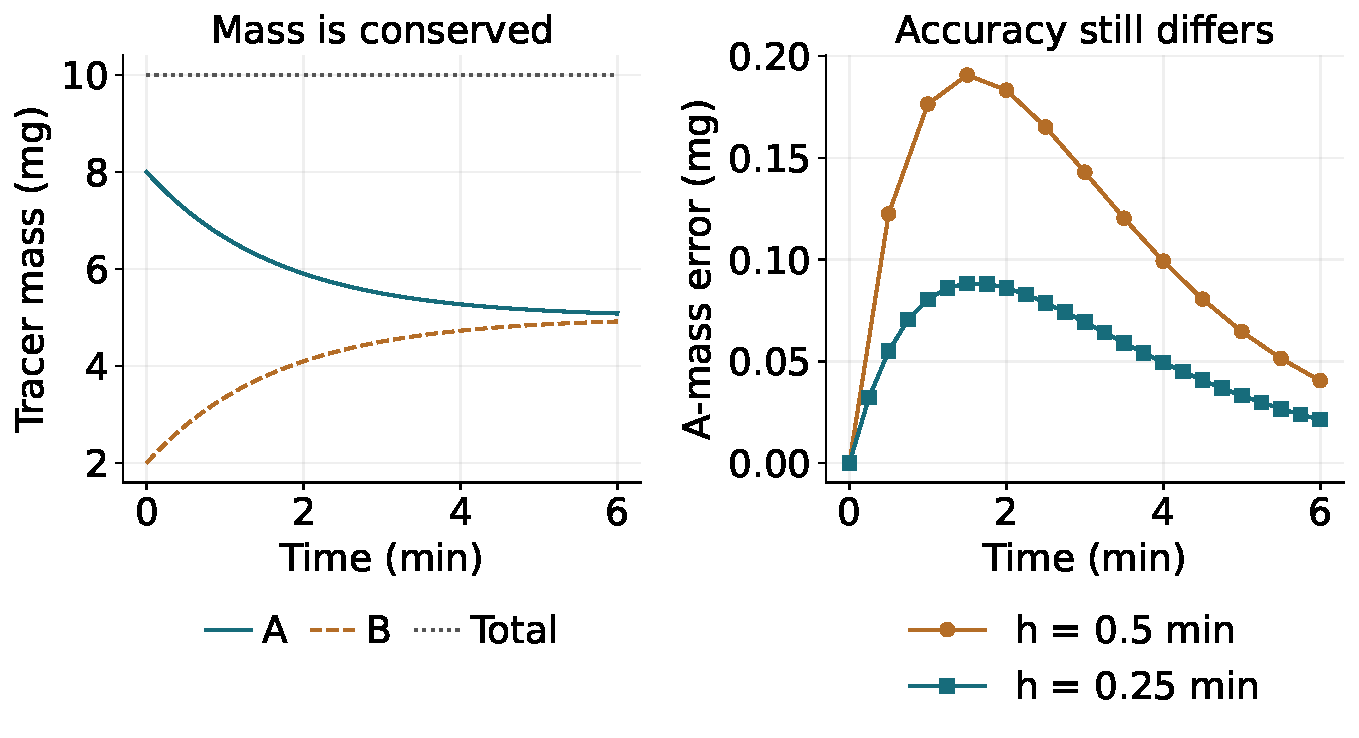
\includegraphics[width=.96\linewidth,height=.57\textheight,keepaspectratio]{exchange-and-error.pdf}\par\smallskip
{\small The two masses sum to 10 mg. Forward Euler preserves this total for both displayed step sizes, yet the individual-state error is smaller with the finer step.}
\end{minipage}\end{center}
\section{Euler stability and positivity}
\hypertarget{note-euler-stability-and-positivity}{}\label{note:euler-stability-and-positivity}
{\small \href{slides.html\#frame=euler-stability-and-positivity\&step=1}{Slides for this section}}\par
Forward Euler preserves the total exactly because the two updates still contain equal and opposite transfers. This conservation says nothing by itself about the accuracy of the difference mode. Positivity of each mass follows when the update is a convex combination of the old masses, giving a step condition that must be examined separately from monotone relaxation.

\[
\begin{pmatrix}m_A^{n+1}\\m_B^{n+1}\end{pmatrix}
=\begin{pmatrix}1-kh&kh\\kh&1-kh\end{pmatrix}
\begin{pmatrix}m_A^n\\m_B^n\end{pmatrix}.
\]

Nonnegative coefficients require $0\leq kh\leq1$.

\subsection*{The difference-mode multiplier}
\[
d_{n+1}=(1-2kh)d_n.
\]

Decay requires $0<kh<1$. Monotone decay requires $0<kh\leq1/2$. A conserved total can coexist with an inaccurate or oscillating state.

The companion uses the stricter condition $2kh\le1$ so the concentration difference decays without sign changes. This monotonicity requirement is stronger than positivity and absolute stability alone.
\section{Step refinement}
\hypertarget{note-step-refinement}{}\label{note:step-refinement}
{\small \href{slides.html\#frame=step-refinement\&step=1}{Slides for this section}}\par
Compare both numerical state trajectories with the exact solution on a common output grid. A mass residual checks cancellation of transfers. A state error checks approximation of the nonzero eigenmode. The two diagnostics should be reported separately.

\[
\epsilon_M=\max_n|m_A^n+m_B^n-10|,
\]

\[
E(h)=\max_n\|m^n-m(t_n)\|_2.
\]
For Euler, $E(h)=O(h)$ under ordinary smoothness assumptions.

\subsection*{A local truncation calculation}
\[
e^{-2kh}=1-2kh+2k^2h^2+O(h^3).
\]

Euler retains only the first two terms. The one-step difference is $O(h^2)$ and the accumulated fixed-time error is $O(h)$.
\begin{center}\begin{minipage}{.98\linewidth}\centering
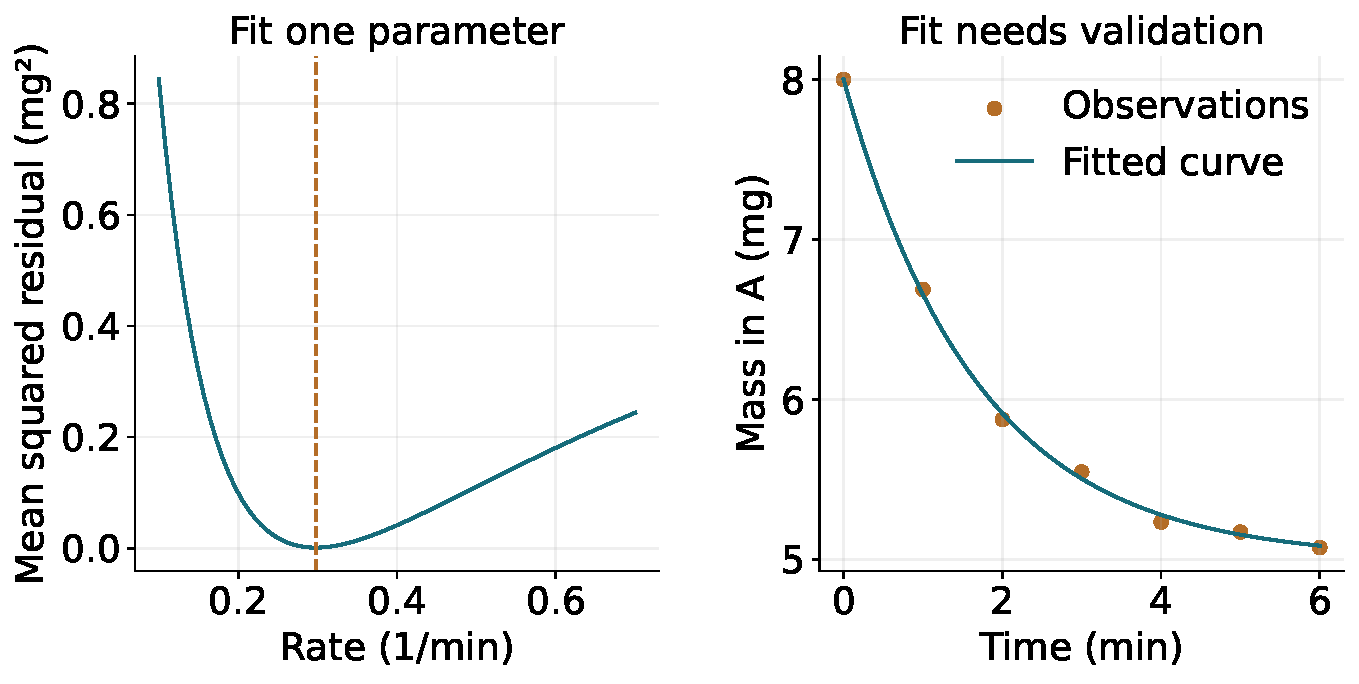
\includegraphics[width=.96\linewidth,height=.57\textheight,keepaspectratio]{parameter-evidence.pdf}\par\smallskip
{\small The fit uses exact model values and seven synthetic perturbed observations of A, keeping parameter residuals separate from numerical integration error. Search bounds are 0.01--1 min$^-$$^1$; the displayed objective window is narrower.}
\end{minipage}\end{center}
\Needspace{10\baselineskip}
\section{Estimating the exchange coefficient}
\hypertarget{note-estimating-the-exchange-coefficient}{}\label{note:estimating-the-exchange-coefficient}
{\small \href{slides.html\#frame=parameter-evidence-figure\&step=1}{Slides for this section}}\par
Suppose only compartment A is observed. With the initial state fixed, fit $k$ by minimizing residuals between the exact model and the measurements. Using the exact formula here keeps parameter-fitting error separate from integration error. Positivity and a declared search interval restrict admissible coefficients.

\[
J(k)=\sum_i[5+3e^{-2kt_i}-y_i]^2,\qquad k>0.
\]

\[
\partial_k m_A(t;k)=-6te^{-2kt}.
\]

\subsection*{Informative observation times}
The initial measurement carries no sensitivity to $k$ when the initial state is fixed. Late measurements approach $5$ mg for every positive $k$.

The magnitude $te^{-2kt}$ is largest at $t=1/(2k)$.
\bigskip
\section*{Exercises}
\par\noindent\begin{minipage}{\linewidth}
\subsection*{P27-3-1. Interpret a sensor solve}
A new observation map gives readings u=\allowbreak{}mA+\allowbreak{}0.5mB and v=\allowbreak{}mB. Measured readings are (7,4) mg-equivalent. Total: 10 points.

\textbf{a} Recover both masses and substitute them into both channels.

\end{minipage}\par\medskip
\textbf{b} State the matrix and vector shapes and residual units.

\textbf{c} If both channels instead measure mA+\allowbreak{}mB, what can and cannot be determined?

\par\noindent\begin{minipage}{\linewidth}
\subsection*{P27-3-2. Transfer and a hand step}
Two equal-volume reservoirs start at 9 and 3 mg with k=\allowbreak{}0.2 min$^-$$^1$. Use an Euler step h=\allowbreak{}0.5 min. Total: 10 points.

\textbf{a} Calculate the initial transfer rate and both derivatives with units.

\end{minipage}\par\medskip
\textbf{b} Calculate the next Euler state and check total mass.

\textbf{c} Find the difference multiplier and state whether the teaching monotonicity condition holds.

\par\noindent\begin{minipage}{\linewidth}
\subsection*{P27-3-3. An invariant is not an accuracy estimate}
Two simulations both preserve a 12 mg total. At one time their A-state errors against a known exact solution are 0.4 and 0.1 mg. Total: 10 points.

\textbf{a} What does conservation establish, and what does it fail to establish?

\end{minipage}\par\medskip
\textbf{b} A coarse step gives the first error and a smaller step gives the second. What bounded conclusion is supported?

\textbf{c} Explain why a library output grid is not necessarily its internal integration grid.

\par\noindent\begin{minipage}{\linewidth}
\subsection*{P27-3-4. What does a fitted rate mean?}
The model's initial masses are known and unequal. A colleague fits k from observations of A. Total: 10 points.

\textbf{a} Why do repeated observations at time zero fail to determine k?

\end{minipage}\par\medskip
\textbf{b} Define a mean squared residual objective and give its units when observations are mg.

\textbf{c} Name one numerical verification check and one independent scientific validation observation.

\section*{References}
\noindent\begin{minipage}{\linewidth}
Original Python Lecture 3. PDF pages 8--13.

\url{https://zanahmad.com/files/scientific-python/Lecture_3__Intro_to_Python.pdf}
\end{minipage}\par\medskip
\noindent\begin{minipage}{\linewidth}
Original Python Lecture 4. PDF pages 9--13.

\url{https://zanahmad.com/files/scientific-python/Lecture_4__Intro_to_Python.pdf}
\end{minipage}\par\medskip
\noindent\begin{minipage}{\linewidth}
SciPy solve\_ivp documentation. Initial-value problem, t\_eval and error tolerance parameters.

\url{https://docs.scipy.org/doc/scipy/reference/generated/scipy.integrate.solve_ivp.html}
\end{minipage}\par\medskip
\noindent\begin{minipage}{\linewidth}
SciPy minimize\_scalar documentation. Bounded scalar minimization and success result.

\url{https://docs.scipy.org/doc/scipy/reference/generated/scipy.optimize.minimize_scalar.html}
\end{minipage}\par\medskip
Python source materials: Phillip Kerger (2023). Course adaptation and additional exposition: Zan Ahmad.

\end{document}
